\section{Our approach}
\label{sec:preproc}

Next, we describe our approach. The algorithm first partitions the mesh into patches that are locally optimized for reduced ACMR.
It then generates a set of index buffers that contain different orderings of these patches. These different orders 
are optimized for reducing overdraw for different keyframes and viewpoints.

\subsection{Generating cache-efficient patches}
We follow the {\em fast linear clustering} approach of~\cite{Sander07} to quickly generate
cache-optimized surface patches of triangles. The basic idea is to first optimize the entire
mesh to reduce ACMR, and then break the output index buffer into contiguous triangle sequences, or patches.
The approach uses a parameter $\lambda$ to regulate the resulting ACMR.
Essentially, the method traverses the order one triangle at a time, and when the ACMR of the current patch 
drops below $\lambda$, it adds a patch break and starts a new patch on the following triangle.
Refer to ~\cite{Sander07} for additional details. 
Lower values of $\lambda$ result in lower overall ACMR, however due to the smaller number of patch breaks, it 
provides less flexibility for patch reordering to reduce overdraw.

\subsection{Generating the index buffers}
Next, we seek to reorder of these cache-optimized patches for overdraw reduction.

\paragraph{Viewpoints}
We assume that the animated model may be viewed from all directions. We first generate a set $V$ of 162 viewpoints that lie on a sphere enclosing the model to represent the potential viewing directions (figure~\ref{fig:modelview}). The viewpoints are computed by subdividing an icosahedron as in~\cite{Nehab06}.  If the viewpoint distribution of the target application differs significantly, a specialized set of viewpoints can be generated.

\begin{figure}[t]
\centering
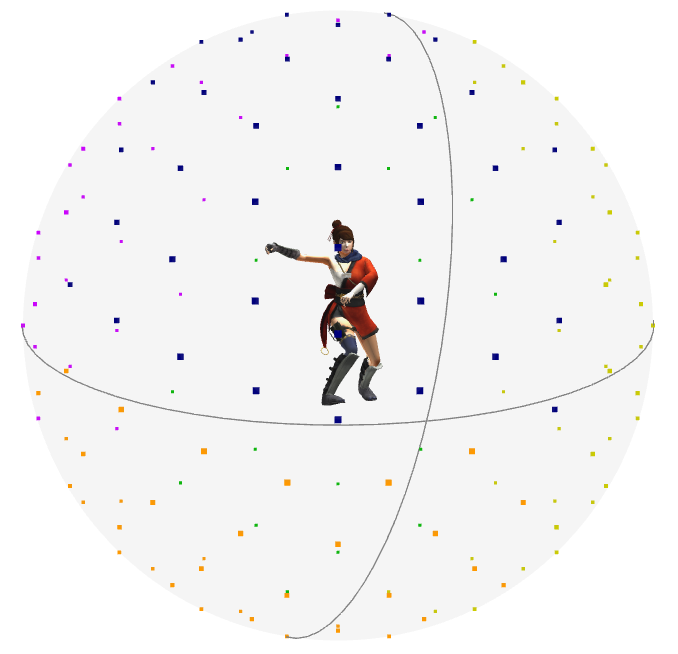
\includegraphics[width = .8\columnwidth]{images/modelview.png}%
\caption{The points represent the vertices from the subdivided icosahedron that were used as viewpoints during clustering. The colors identify their clusters.}
\label{fig:modelview}
\end{figure}

\paragraph{Clustering}
A single order that is suitable for all animation keyframes when viewed from any viewpoint cannot satisfactorily reduce overdraw (see single cluster results in section~\ref{sec:results}).
We instead create $k$ clusters of (keyframe, viewpoint) pairs that can share index buffers. This results in a total of $k$ index buffers. At runtime, the rendering algorithm picks the appropriate one based on the current viewpoint and keyframe. 

We are given a set of viewpoints $V$ and a set of keyframes $F$. Our approach must consider every possible keyframe viewed from every possible direction. Since $|V| = 162$ and $30 \leq |F| \leq 70$ for our example animations, the total number of nodes (i.e., keyframe and viewpoint combinations) is in the thousands.

We seek to find a partitioning of all nodes that yields low overdraw with a small number of index buffers. Our approach is based on k-means clustering~\citep{MacQueen67}. The algorithm alternates between two steps, one which assigns nodes to clusters, and one which computes a new index buffer for each cluster.

\paragraph{Bootstrapping}
The algorithm is initialized by choosing $k$ random nodes and creating an initial index buffer for each of them by sorting the patches in front-to-back order (i.e., by increasing distance between the patch centroid and the node viewpoint). These $k$ buffers represent our initial $k$ clusters. The choice of $k$ is discussed in the results section.

\paragraph{Step 1: Node assignment} Each node is assigned to the cluster whose index buffer results in the lowest overdraw when used to render that keyframe from that particular viewpoint. This is accomplished by rendering the scene using each of the $k$ candidate index buffers and using hardware occlusion queries to read back the overdraw results.

\paragraph{Step 2: Index buffer computation} For each cluster, we compute a new triangle order with reduced average overdraw for all of its currently assigned nodes. We accomplish this by creating an order that roughly sorts the patches from front-to-back. 
Sorting the patches from front-to-back is straightforward if we only consider one node (i.e., a single keyframe from a single viewpoint). However, in this case, the order must be suitable for all the nodes assigned to the cluster. We accomplish this by integrating the distances between viewpoints and patch centroids over all of the nodes in the cluster. We then create a single global order that sorts the patches in front-to-back order based on their integrated patch distances. Patches whose triangles are all backfacing are ignored in the distance computation, and the integrated distance is normalized based on the number of nodes in which it is visible.




\subsection{Runtime selection}
When rendering the model, the target application has to choose between one of the $k$ index buffers. This is accomplished by using a lookup table indexed by keyframe and viewpoint. For simplicity, we index viewpoints based on polar and azimuth angles $(\theta, \phi)$ (we use values from the closest original viewpoint when populating the table). While this distribution is less uniform than the subdivided icosahedron, it is only used to store the index buffer IDs for the purpose of simplifying the lookup at runtime. The time required for the lookup is negligible since it is only a single lookup for the entire model. The lookup parameters $f$, $\theta$, and $\phi$ are rounded to the nearest valid parameter values.


\ignore{
When rendering the model, the target application has to choose between one of the $k$ index buffers. This is accomplished by using a lookup ${\bf IBid}[f, \theta_v, \phi_v]$ indexed by keyframe $f$ and viewpoint $v$. 
The vertices from the subdivided icosahedron (i.e., viewpoints) are grouped by their polar angles, resulting in $n$ lists $L_i$, of vertices that share the same polar angle $\theta_i$ ($n = 13$ in our case).
Within each list, the vertices are sorted by azimuth angle $\phi$. Polar angles of the lists are uniformly separated by $\pi / (n-1)$, and the azimuth angles within each list $L_i$ are uniformly separated by $2 \pi / (|L_i|-1)$. Thus, given $\theta_v,\phi_v$, we can determine the closest vertex to the queried viewpoint in constant time. The overall time required for this lookup is negligible since it is only a single lookup for each rendered model.
}
